Nel contesto della gestione dell'\Gls{atm}, lo spazio aereo viene modellato attraverso un insieme di entità geometriche e funzionali che ne descrivono l’organizzazione e le modalità operative. Al fine di rappresentare in maniera accurata le configurazioni spaziali e temporali utilizzate nella gestione della capacità e del controllo del traffico, è utile introdurre alcune definizioni fondamentali che costituiscono la base del modello adottato da \citet{eurocontrol2025}.

\section{Definizioni preliminari}
Lo spazio aereo è rappresentato attraverso unità di controllo elementari che possono essere aggregate su più livelli, secondo gli schemi descritti nelle sottosezioni che seguono. In questa sezione si introducono le principali entità geometriche e funzionali del modello, che verranno poi richiamate nella definizione delle metriche di capacità e nelle formulazioni di ottimizzazione.

\subsection{Airblock}
L’airblock è l’unità spaziale di base del modello. Esso è definito come un poligono chiuso in due dimensioni (2D), rappresentato come una sequenza ordinata di punti in coordinate geografiche. Ogni airblock delimita una porzione dello spazio aereo e costituisce la tessera elementare (o tassello) del mosaico bidimensionale che modella il dominio orizzontale dello spazio aereo. L’insieme completo degli airblock fornisce dunque una partizione esaustiva e non sovrapposta dello spazio aereo orizzontale.
\clearpage
\subsection{Settore elementare (\emph{elementary sector})}
\label{subsec:settore-elementare}
Il settore elementare (\emph{elementary sector}) è un volume tridimensionale ottenuto associando a un airblock un intervallo di livelli di volo. Ogni settore è identificato dalla seguente tripletta, che ne descrive la struttura spaziale:
\begin{equation*}
    (\text{airblock}, \text{\acrshort{fl}}_{\min}, \text{\acrshort{fl}}_{\max})
\end{equation*}
Tale settore rappresenta l’unità minima di gestione del traffico aereo in ambito operativo e viene utilizzato nella pianificazione della capacità.

\subsection{Settore collassato (\emph{collapsed sector})}
\label{subsec:settore-collassato}

Il settore collassato (\emph{collapsed sector}) è un volume dello spazio aereo ottenuto mediante l’unione di almeno un settore elementare. Tale aggregazione ha lo scopo di adattare dinamicamente la configurazione dello spazio aereo in funzione del volume di traffico atteso e della disponibilità delle risorse di controllo.

In particolare, affinché le configurazioni collassate siano attuabili senza generare eccessiva complessità operativa, devono essere rispettati i seguenti vincoli:
\DisablePunct
\begin{itemize}
  \item {\bf Convessità} (cfr.~Figura~\ref{fig:convexity}): ogni settore collassato deve avere una forma convessa, in modo da limitare la complessità geometrica e ridurre i punti di possibile conflitto all’interno dello spazio aereo, semplificando il monitoraggio radar e le manovre dei controllori;
  \item {\bf Tempo minimo di permanenza} (cfr.~Figura~\ref{fig:minstay}): un settore collassato, una volta attivato, deve rimanere operativo per almeno \(t_p\) intervalli di tempo, al fine di evitare cambi troppo rapidi che comporterebbero numerosi handover (cioè il trasferimento della responsabilità di sorveglianza e comunicazione di un aeromobile da un settore di spazio aereo a un altro) e un sovraccarico procedurale per i centri di controllo;
 \clearpage
  \begin{figure}[H]
    \centering
    \begin{subfigure}[b]{0.45\textwidth}
      \centering
      \begin{tikzpicture}[scale=0.8]
  \filldraw[fill=gray!20, draw=black, line width=0.5pt]
    (0,0) rectangle (8,6);

  \path[name path=s1border]
    (0,6) -- (8,6) -- (6.4,1) -- (4.8,4) -- (3.2,1) -- cycle;

  \filldraw[fill=yellow!50]
    (0,6) -- (8,6) -- (6.4,1) -- (4.8,4) -- (3.2,1) -- cycle;

  \draw[name path=centerline, draw=green!70!black, line width=0.5pt]
    (0,3) -- (8,3);

  \path[name intersections={of=s1border and centerline, by={I1,I2,I3,I4}}];

  \foreach \pt in {I1,I2,I3,I4} {
    \draw[draw=red, line width=1pt] (\pt) circle[radius=0.3];
  }

  \node at (4.2,4.8) {$S_1$};
  \node at (4.2,1.2) {$S_2$};
\end{tikzpicture}
      \subcaption{Convessità: l’aeromobile attraversa quattro volte i confini di \(S_1\), situazione non ammessa.}
      \label{fig:convexity}
    \end{subfigure}\hfill
    \begin{subfigure}[b]{0.45\textwidth}
      \centering
      \begin{tikzpicture}[scale=0.8]
  \filldraw[fill=gray!20, draw=black, line width=0.5pt]
    (0,0) rectangle (8,6);

  \path[name path=wedgeborder]
    (3.2,6) -- (4.8,6) -- (4,0) -- cycle;

  \filldraw[fill=yellow!50, draw=black, line width=0.5pt]
    (3.2,6) -- (4.8,6) -- (4,1.5) -- cycle;

  \draw[draw=black, line width=0.5pt] (4,1.5) -- (4,0);
    
  \draw[name path=centerline, draw=green!70!black, line width=0.5pt]
    (1.2,3) -- (6.8,3);
  \fill[green!70!black] (1.2,3) circle (2pt);
  \draw[draw=green!70!black, line width=0.5pt] (1.2,3) -- (0,4);
  \draw[draw=green!70!black, line width=0.5pt] (1.2,3) -- (0,2);
  \draw[draw=green!70!black, line width=0.5pt] (6.8,3) -- (8,4);
  \fill[green!70!black] (6.8,3) circle (2pt);
  \draw[draw=green!70!black, line width=0.5pt] (6.8,3) -- (8,2);

  \path[name intersections={of=wedgeborder and centerline, by={I1,I2}}];

  \foreach \pt in {I1,I2} {
    \draw[draw=red, line width=1pt] (\pt) circle[radius=0.3];
  }

  \node at (2,1.2) {$S_1$};
  \node at (4,4.5) {$S_2$};
  \node at (6,1.2) {$S_3$};
\end{tikzpicture}

      \subcaption{Tempo minimo: il periodo di attivazione di \(S_2\) è inferiore a \(t_p\), con frequenti passaggi di responsabilità.}
      \label{fig:minstay}
    \end{subfigure}
    \caption{Vincoli di convessità (a) e tempo minimo di permanenza nei settori (b) collassati \cite{treimuth2018dynamic}.}
    \label{fig:constraints_ab}
  \end{figure}

  \item {\bf Connettività} (cfr.~Figura~\ref{fig:connectivity}): il settore collassato deve costituire un’unica regione connessa, senza parti disgiunte, affinché l’insieme di blocchi aerei aggregati risulti gestibile come un unico volume di responsabilità;
  \item {\bf Rispetto dei confini} (cfr.~Figura~\ref{fig:boundary}): è necessario mantenere una distanza minima dai confini degli \gls{acc} adiacenti, garantendo buffer spaziali che facilitino il coordinamento e riducano il rischio di conflitti in prossimità dei limiti di settore.
  \begin{figure}[htbp]
    \centering
    \begin{subfigure}[b]{0.45\textwidth}
      \centering
      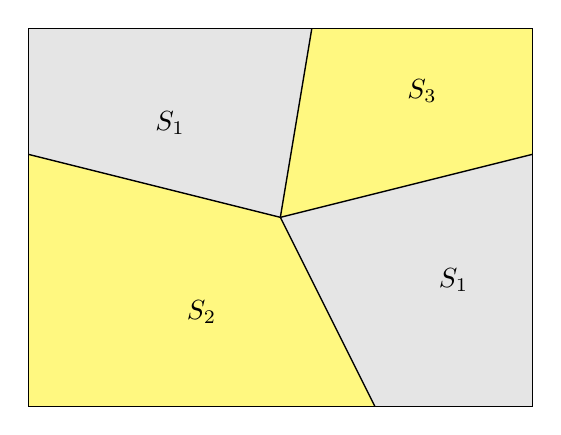
\begin{tikzpicture}[scale=0.8]
  %–– Regioni ––
  % S1 sinistro
  \fill[gray!20]
    (4,3) -- (0,4) -- (0,6) -- (4.5,6) -- cycle;
  % S3 (giallo)
  \fill[yellow!50]
    (4,3) -- (4.5,6) -- (8,6) -- (8,4) -- cycle;
  % S1 destro
  \fill[gray!20]
    (4,3) -- (8,4) -- (8,0) -- (5.5,0) -- cycle;
  % S2 (azzurro)
  \fill[yellow!50]
    (4,3) -- (5.5,0) -- (0,0) -- (0,4) -- cycle;

  %–– Confini interni spessi blu ––
  \draw[black, line width=0.5pt] (4,3) -- (0,4);
  \draw[black, line width=0.5pt] (4,3) -- (4.5,6);
  \draw[black, line width=0.5pt] (4,3) -- (8,4);
  \draw[black, line width=0.5pt] (4,3) -- (5.5,0);

  %–– Bordo esterno ––
  \draw[black, line width=0.5pt] (0,0) rectangle (8,6);

  %–– Etichette ––
  \node at (2.25,4.5) {$S_1$};
  \node at (2.75,1.5) {$S_2$};
  \node at (6.25,5) {$S_3$};
  \node at (6.75,2) {$S_1$};
\end{tikzpicture}

      \subcaption{Connettività: il settore risulta suddiviso in due componenti disgiunte.}
      \label{fig:connectivity}
    \end{subfigure}\hfill
    \begin{subfigure}[b]{0.45\textwidth}
      \centering
      \begin{tikzpicture}[scale=0.8]
  %--- coordinate principali
  \coordinate (A) at (1,3);
  \coordinate (B) at (3.2,3);
  \coordinate (C) at (6.5,4.2);
  \coordinate (D) at (6,1.5);
  \coordinate (L) at (2.5,6);
  \coordinate (V) at (4,4.5);
  \coordinate (R) at (5.5,6);

  %--- aree colorate
  \fill[gray!20]   (0,0) -- (0,6) -- (L) -- (V) -- (4,0) -- cycle;
  \fill[gray!20]  (4,0) -- (V) -- (R) -- (8,6) -- (8,0) -- cycle;
  \fill[yellow!50] (L) -- (V) -- (R) -- cycle;

  %--- bordi saturi
  \draw[black,line width=0.5pt] (L) -- (V) -- (R);
  \draw[black,line width=0.5pt] (V) -- (4,0);

  %--- contorno esterno
  \draw[black, line width=0.5pt] (0,0) rectangle (8,6);

  %--- segmenti sottili verso 2 e 4
  \draw (B) -- (C);
  \draw (B) -- (D);
  \draw (A) -- (B);

  %--- vettori con aereo all'inizio e freccia alla fine
  \draw[green!70!black,very thick,->, shorten >=20pt]
    (A) node[sloped,allow upside down,above,inner sep=0pt,
             transform shape,rotate=-45, yshift=10pt] {}
    -- ($(A)!0.8!(B)$);

  \draw[green!70!black,very thick,->, shorten >=40pt]
    (C) node[sloped,allow upside down,above,inner sep=0pt,
             transform shape,rotate=160, yshift=-10pt, xshift=15pt] {}
    -- ($(C)!0.8!(B)$);
    
  %--- siti e cerchio rosso
  \draw[fill=black] (A) circle (2pt) node[left]  {1};
  \draw[fill=black] (B) circle (2pt) node[below right, yshift=-5pt] {3};
  \draw[fill=black] (C) circle (2pt) node[right] {2};
  \draw[fill=black] (D) circle (2pt) node[below] {4};
  \draw[red,thick]   (B) circle (8pt);

  %--- etichette dei settori
  \node at (1.5,1)   {$S_1$};
  \node at (6.5,2.5) {$S_2$};
  \node at (4,5.5)   {$S_3$};
\end{tikzpicture}
      \subcaption{Confini: attraversamenti troppo vicini al bordo, ridotto buffer operativo.}
      \label{fig:boundary}
    \end{subfigure}
    \caption{Vincoli di connettività (a) e rispetto dei confini nei settori (b) collassati \cite{treimuth2018dynamic}.}
    \label{fig:constraints_cd}
  \end{figure}
\end{itemize}
\EnablePunct
\subsection{Control Area}
La \gls{cta} costituisce una porzione contigua e coerente di spazio aereo, ottenuta attraverso l’aggregazione di uno o più settori, siano essi elementari o collassati. Essa si configura come una struttura di ordine superiore all’interno dell’architettura gerarchica dello spazio aereo, che include, su livelli inferiori, gli airblocks, i settori e gli airspace.
Dal punto di vista funzionale, la \acrshort{cta} rappresenta un'entità organizzativa concepita sia per scopi operativi sia per esigenze analitiche. In particolare, essa consente di modellare un’area omogenea in termini di attribuzione della capacità e di gestione del traffico aereo. Ogni \acrshort{cta} è affidata alla supervisione di un \Gls{acc}, gestito da un \Gls{ansp}, il quale è responsabile dell’erogazione dei servizi di controllo all’interno dei volumi di spazio assegnati.

Una rappresentazione della \gls{cta} e dei settori collassati è fornita nella Figura~\ref{fig:cta}, derivata da \cite{ehrencrona2014} come esito del lavoro di ricerca sui metodi di formazione delle configurazioni.

\begin{figure}[H]
  \centering
  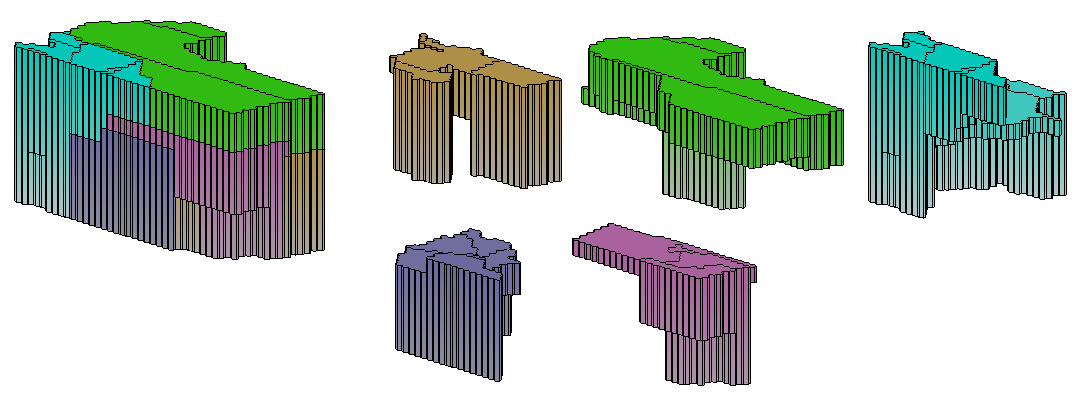
\includegraphics[width=0.9\textwidth]{chapters/ch1/img/madrid_south_ACC}
  \caption{Un esempio di \acrshort{cta}: a destra la \acrshort{cta} di ``Madrid South'', a sinistra la sua decomposizione in settori collassati \cite{ehrencrona2014}.}
  \label{fig:cta}
\end{figure}


\subsection{Flight Information Region}

La \gls{fir} costituisce la principale suddivisione standardizzata dello spazio aereo, istituita per garantire i servizi di informazione volo e di allarme. Tali servizi comprendono l'assistenza alla navigazione sicura ed efficiente, oltre alla gestione delle emergenze che coinvolgono gli aeromobili noti.

Le \acrshort{fir} corrispondono generalmente ai confini nazionali (cfr.\ Figura~\ref{fig:svizzera_fir}), sebbene possano estendersi su più stati o suddividersi all'interno di ampie nazioni (cfr.\ Figura~\ref{fig:italia_fir}). Ogni \acrshort{fir} rappresenta un'entità stabile e permanente, definita su base strategica e soggetta a modifiche solo in casi eccezionali.
\clearpage
\begin{figure}[H]
  \centering
  \begin{minipage}[t]{0.47\textwidth}
    \centering
    \begin{overpic}[width=\linewidth]{chapters/ch1/img/italia_fir}
      \put(17,78){\color{black}\tiny{LIMMFIR}}
      \put(36,36){\color{black}\tiny{LIRRFIR}}
      \put(58,47){\color{black}\tiny{LIBBFIR}}
    \end{overpic}
    \caption{Confini delle FIR italiane LIRRFIR, LIMMFIR e LIBBFIR nello spazio aereo inferiore (Lower Airspace).}
    \label{fig:italia_fir}
  \end{minipage}
  \hfill
  \begin{minipage}[t]{0.47\textwidth}
    \centering 
    \raisebox{15mm}[0pt][0pt]{%
      \begin{overpic}[width=\linewidth]{chapters/ch1/img/svizzera_fir}
        \put(45,32){\color{black}\tiny{LSASFIR}}
      \end{overpic}%
    }
    \caption{Confine della FIR svizzera LSASFIR nello spazio aereo inferiore (Lower Airspace).}
    \label{fig:svizzera_fir}
  \end{minipage}
\end{figure}

% ------ da togliere
\iffalse
\subsubsection{ATC Unit Airspace}

L'\gls{aua} è un volume di spazio aereo posto sotto la responsabilità di una specifica unità di controllo del traffico aereo, come una torre di controllo aeroportuale o una \acrshort{cta}. All'interno di ciascun \acrshort{aua} vengono garantiti i servizi di gestione e sorveglianza del traffico aereo, assicurando la sicurezza e la regolarità delle operazioni.

Gli \acrshort{aua} sono strutture operative relativamente stabili, organizzate per supportare la divisione gerarchica e funzionale dello spazio aereo.
\fi
% ------

%Diversamente dalle \acrshort{fir}, i settori collassati costituiscono configurazioni dinamiche e temporanee dello spazio aereo. Essi derivano dall'aggregazione o dalla divisione di settori elementari in risposta a esigenze operative contingenti, come le variazioni giornaliere nel volume di traffico.

\section{Dynamic Airspace Configuration}
La gestione dello spazio aereo avviene secondo logiche dinamiche e flessibili, guidate dal principio del \acrfull{fua}, che prevede l’utilizzo ottimizzato delle risorse spaziali in risposta alle variazioni previste nel traffico e integra in modo coordinato le esigenze civili e militari~\citep{ec2150_2005,eurocontrol_ans_fua}.

In ambito operativo, ciò si realizza attraverso configurazioni settoriali che evolvono nel corso della giornata. Ogni configurazione è costituita da una combinazione di settori attivi (vedi Sezioni~\ref{subsec:settore-elementare} e~\ref{subsec:settore-collassato}), selezionati secondo un \emph{opening scheme} che ne determina la temporizzazione. Chiamiamo \emph{opening scheme} di un dato \gls{acc}, per un dato giorno, la descrizione delle diverse configurazioni che si susseguono nel corso della giornata~\citep{opscheme1, opscheme2}. A ciascun settore attivo è associata una capacità nominale, definita come il numero massimo di voli che possono essere gestiti per unità di tempo, determinata sulla base della complessità operativa e delle risorse disponibili.

Il problema del \acrfull{dac} consiste nel determinare la sequenza ottimale delle configurazioni dello spazio aereo in un intervallo temporale, con l'obiettivo di minimizzare l’eccedenza della domanda di traffico rispetto alla capacità disponibile. Nel contesto operativo utilizzato in \citep{galeazzo2024integer}, il problema assume di disporre di:
\begin{itemize}
    \item un insieme finito di configurazioni ammissibili
    \item la domanda di traffico prevista su ciascun settore e la sua evoluzione temporale
    \item la capacità nominale di ciascun settore
\end{itemize}
% TODO si ripete quello scritto sopra?
Data tale situazione operativa, l'obiettivo del \acrshort{dac} diventa quello di individuare la successione temporale delle configurazioni che consenta di gestire al meglio il traffico atteso, minimizzando eventuali sovraccarichi (eccessi di domanda) e rispettando vincoli operativi quali:
\begin{itemize}
    \item l’intervallo minimo di permanenza (permanence) in ogni configurazione, evitando cambiamenti frequenti e complessi per i controllori
    \item l’intervallo di quiescenza (quiescence), ovvero il tempo minimo che deve trascorrere prima di poter riattivare una configurazione precedentemente disattivata
    \item la compatibilità tra configurazioni consecutive, in modo da consentire transizioni fluide
\end{itemize}


Tale problema può essere formulato matematicamente mediante un modello di \Gls{ilp}, come formulato in \cite{galeazzo2024integer} e riportato nella sezione seguente.

\subsection{Formulazione matematica}
La formulazione matematica del problema del \gls{dac} può essere rappresentata attraverso un modello di \gls{ilp} introdotto da \citet{galeazzo2024integer}. Tale modello consente di determinare la successione ottimale delle configurazioni spaziali del traffico aereo lungo un orizzonte temporale discreto, minimizzando l'eccesso di domanda rispetto alla capacità disponibile, nel rispetto dei vincoli operativi richiesti per una gestione sicura ed efficiente del traffico aereo.\\\\
Si introducono di seguito le notazioni adottate nel modello:
\begin{itemize}
    \item $T$: insieme ordinato degli intervalli temporali considerati, $T = \{1, \dots, |T|\}$
    \item $C$: insieme delle configurazioni spaziali dello spazio aereo ammissibili
    \item $C^t \subseteq C$: insieme delle configurazioni disponibili nel periodo temporale $t$
    \item $E^c_t$: eccesso di domanda non negativo della configurazione $c \in C^t$ nel periodo temporale $t$
    \item $t_p$: intervallo minimo di permanenza di una configurazione
    \item $t_q$: intervallo minimo di quiescenza, ossia tempo minimo tra due attivazioni successive della stessa configurazione
    \item $C_{c}^{t+1}$: insieme delle configurazioni che possono seguire immediatamente la configurazione $c$ nel periodo temporale successivo $t+1$
\end{itemize}
    Le variabili decisionali sono definite come segue:
    \begin{itemize}
        \item $x^c_t$: variabile binaria che assume valore 1 se la configurazione $c \in C^t$ è attiva nel periodo $t$, e 0 altrimenti
        \item $s^c_t$: variabile binaria che assume valore 1 se avviene una transizione alla configurazione $c$ al tempo $t$ (ossia $c$ è attiva al periodo $t$ e non al periodo $t-1$), e 0 altrimenti
    \end{itemize}
    Formalmente, il modello ILP può essere espresso nel modo seguente:
    \begin{subequations}\label{eq:modello}
    \begin{align}
    \min\;& \sum_{t \in T} E^c_t\, x^c_{t} \label{eq:objfun}\\
    \text{s.t.}\;& \sum_{c \in C_t} x^c_{t} = 1
        && \forall\,t \in T \label{eq:unicaconf}\\
    & x^c_{t} - \sum_{c' \in C_c^{t+1}} x^{c'}_{t+1} \le 0
        && \forall\,c \in C^t,\ \forall\,t \in T \label{eq:transizioni}\\
    & \sum_{\tau = t}^{t+t_p-1} \sum_{c \in C^{\tau}} s^c_{\tau} \le 1
        && \forall\,t \in T \label{eq:minpermanenza}\\
    & x^c_t - x^c_{t-1} \le s_t^c 
        && \forall\,c \in C^t,\ \forall\,t \in T \label{eq:transizione}\\
    & x^c_t + \sum_{\tau = t +1}^{t+t_q} s^c_{\tau} \le 1
        && \forall\,c \in C^t,\ \forall\,t \in T \label{eq:quiescenza}\\
    & x^c_t,\, s_t^c \in \{0,1\}
        && \forall\,c \in C^t,\ \forall\,t \in T \label{eq:binaria}
    \end{align}
    \end{subequations}

I vincoli operativi del modello ILP sono interpretati come segue. Il vincolo (\ref{eq:unicaconf}) assicura l’unicità della configurazione attiva in ciascun periodo temporale. Il vincolo (\ref{eq:transizioni}) definisce le condizioni di transizione ammissibili tra configurazioni consecutive. Il vincolo (\ref{eq:minpermanenza}) impone che, una volta attivata, una configurazione resti attiva per almeno $t_p$ periodi consecutivi, prevenendo transizioni troppo frequenti. Il vincolo (\ref{eq:quiescenza}) garantisce che una configurazione disattivata non venga riattivata prima del trascorrere del periodo minimo di quiescenza $t_q$. Infine, il vincolo (\ref{eq:transizione}) collega le variabili decisionali $x^c_t$ e $s^c_t$, registrando esplicitamente l’attivazione di una configurazione.